\documentclass[11pt,spanish]{article} % Tipo y tamaño de letra del documento.

\input{preamble.tex} 

\newcommand{\tnum}{2 y 3} % reemplace 2 por el número de la tarea
\newcommand{\sem}{2025-1} % reemplace 2024-2 por el semestre correspondiente
\newcommand{\campus}{San Joaquín \\ Santiago} % reemplace Casa Central por el campus correspondiente
\newcommand{\rolusm}{202273521-K} % reemplace 2025073100-1 por su rol
\newcommand{\namestudent}{David Kripper} % reemplace Al Goritmo Pérez por su nombre

\headheight=14pt
\linespread{1.3}
\author{\namestudent}
\pagestyle{fancy}
\fancyhf{}%
\fancyfoot[R]{ \namestudent \\ \rolusm}
\fancyfoot[L]{Campus \campus} 
\fancyfoot[C]{\thepage}
\rhead{2025-1}
\lhead{INF-221}
\renewcommand{\headrulewidth}{0.4pt}
\renewcommand{\footrulewidth}{0.4pt}
\newbool{programs}
\boolfalse{programs}
\chead{REPORTE TAREA \tnum~}



\title{
  \huge
  \textbf{REPORTE TAREA \tnum~ \\ ALGORITMOS Y COMPLEJIDAD} \\[1ex]
  \emph{\textquote{Encontrando Diferencias entre dos Secuencias}}
  }

  
\date{
  \small
  \today\\
  \currenttime
}




\begin{document}
\maketitle
\thispagestyle{fancy} 
\vspace{-1.0\baselineskip}




\begin{abstract}
  \textit{ 
    Este trabajo aborda el problema de detectar diferencias entre dos secuencias de texto mediante la métrica de la subsecuencia común más larga (LCS). Se comparan dos paradigmas: fuerza bruta, que examina todas las subsecuencias posibles y garantiza la corrección a costa de un crecimiento exponencial, y programación dinámica, que almacena resultados intermedios y reduce la complejidad. Las implementaciones en C++ emplean la biblioteca \texttt{chrono} para medir tiempos y scripts en Python para generar casos de prueba y gráficar resultados. En un MacBook Air M2, la fuerza bruta pasa de microsegundos a más de 40 minutos cuando $n>17$, mientras que la programación dinámica mantiene tiempos del orden de $10^{-5}$ segundos en todo el rango. La evidencia valida la teoría: la fuerza bruta solo es viable en instancias sumamente pequeñas, mientras que la programación dinámica ofrece una solución práctica y escalable para aplicaciones de procesamiento de lenguaje natural, bioinformática y corrección ortográfica.
  }
     
\end{abstract}

\setcounter{tocdepth}{1}
\tableofcontents


\newpage
\section{Introducción}
El presente trabajo se situa en el campo del Análisis y Diseño de Algoritmos en Ciencias de la Computación, un área fundamental para resolver problemas computacionales de manera eficaz y eficiente. Dentro de este campo, los problemas de edición y comparación de cadenas de texto han recibido gran atención, especialmente en aplicaciones que requieren medir similitudes entre secuencias, como el procesamiento de lenguaje natural, la bioinformática \cite{contreras2018algoritmos} y la corrección ortográfica. Entre las distintas métricas para medir similitud o diferencia entre secuencias, el análisis de la subsecuencia común más larga (LCS, por sus siglas en inglés) destaca como una herramienta fundamental.

\vspace{0.5 cm}

Una de las estrategias más utilizadas para comparar cadenas es el uso de la subsecuencia común más larga, la cual permite identificar los segmentos que se comparten entre dos secuencias. A partir de la LCS, es posible deducir los fragmentos que difieren entre ambas, lo que permite no solo cuantificar su diferencia sino también obtener una representación visual de estas mismas.

\vspace{0.5 cm}

El propósito de este informe es estudiar y comparar dos enfoques algorítmicos para resolver este problema: el método de fuerza bruta, basado en una búsqueda exhaustiva de todas las subsecuencias comunes, y el método de programación dinámica, que optimiza la búsqueda al ir recordando lo que ya ha calculado, en lugar de volver a hacerlo desde cero. Ambos algoritmos serán evaluados en cuanto a su eficiencia y efectividad para detectar las diferencias entre dos cadenas de texto, analizando cómo escalan en tiempo frente a entradas de diferentes tamaños.

\vspace{0.5 cm}

Este estudio permite introducir conceptos avanzados como el uso de programación dinámica para optimizar procesos combinatorios, y explorar las ventajas y limitaciones de los enfoques de fuerza bruta frente a técnicas algorítmicas más eficientes. El informe tiene como objetivo proporcionar una visión tanto práctica como teórica de cada paradigma, ofreciendo una base sólida para el análisis de algoritmos en contextos donde la comparación entre secuencias es una operación fundamental.


\newpage
\section{Diseño y Análisis de Algoritmos} 
En este trabajo se analizan dos enfoques fundamentales para resolver el problema de detección de diferencias entre secuencias de texto a partir de la subsecuencia común más larga: el enfoque de fuerza bruta y el de programación dinámica. Ambos algoritmos abordan el mismo objetivo pero lo hacen desde perspectivas distintas, cada una con sus ventajas y limitaciones en cuanto a eficiencia, escalabilidad y complejidad de implementación.

\vspace{0.5 cm}

El enfoque de fuerza bruta se basa en la exploración exhaustiva de todas las posibles subsecuencias comunes entre dos cadenas, utilizando técnicas de backtracking. Esta estrategia permite encontrar la subsecuencia común más larga probando cada combinación posible, lo que asegura una solución correcta, aunque a un alto costo computacional. Este método es útil para comprender el comportamiento del problema en instancias pequeñas, ya que considera todos los caminos posibles. Sin embargo, su complejidad crece de forma exponencial con el tamaño de las cadenas, lo que limita seriamente su aplicabilidad a casos reales de gran tamaño.

\vspace{0.5 cm}

Por su parte, el enfoque de programación dinámica resuelve el mismo problema de manera mucho más eficiente. Se basa en dividir el problema en subproblemas más pequeños y almacenar los resultados intermedios. Esto evita el cálculo repetido y mejora considerablemente el tiempo de ejecución. Este enfoque permite escalar a instancias de mayor tamaño, manteniendo su complejidad, lo que lo hace particularmente adecuado para contextos prácticos como la comparación de documentos o secuencias biológicas.

\vspace{0.5 cm}

A continuación, se presenta un análisis detallado de cada algoritmo. Este análisis permitirá comparar ambos métodos y evidenciar por qué la programación dinámica resulta más adecuada para instancias grandes, sin dejar de valorar lo que ofrece la implementación por fuerza bruta.

\subsection{Fuerza Bruta}

La solución de fuerza bruta desarrollada en esta tarea \cite{GfG2025LCS} \cite{Programiz2025LCS} busca identificar las diferencias entre dos secuencias de texto a partir de la subsecuencia común más larga (LCS, por sus siglas en inglés). Para ello, el algoritmo explora exhaustivamente todas las posibles subsecuencias comunes entre dos cadenas, con el fin de encontrar aquella de mayor longitud. Esta subsecuencia se utiliza posteriormente para determinar los fragmentos que difieren entre ambas cadenas. Debido a la naturaleza exhaustiva de este enfoque, el algoritmo resulta poco eficiente cuando se trabaja con cadenas largas.

\vspace{0.5 cm}

La solución se implementa mediante una función recursiva que explora todas las combinaciones posibles de caracteres compartidos entre las dos cadenas. El algoritmo comienza comparando los primeros caracteres de ambas cadenas. Si coinciden, se agregan a la subsecuencia común y se continúa con los siguientes índices. En caso contrario, se realizan dos llamadas recursivas: una avanzando en la primera cadena y otra avanzando en la segunda, evaluando así todas las posibilidades. Una vez obtenida la LCS, se recorre nuevamente cada cadena para identificar los bloques que no pertenecen a dicha subsecuencia, generando así los pares de substrings que representan las diferencias entre ambas.

\vspace{0.5 cm}

Este enfoque garantiza una solución correcta, ya que evalúa todas las opciones posibles para obtener la LCS. Sin embargo, su principal desventaja es el alto costo computacional. La complejidad temporal del algoritmo es exponencial, ya que en el peor de los casos el número de llamadas recursivas crece de manera combinatoria. Para dos cadenas de longitudes \texttt{n} y \texttt{m}, la complejidad temporal se puede expresar de la siguiente manera: \[O(2^{\max(n, m)})\] Esto se debe a que cada posición puede generar múltiples caminos posibles según las decisiones tomadas. Como consecuencia, el enfoque de fuerza bruta se vuelve impractico e infructifero para entradas largas, siendo útil únicamente para analizar instancias pequeñas.

\vspace{0.5 cm}

En cuanto al análisis espacial, el principal consumo de memoria proviene de la pila de llamadas recursivas. Cada vez que el algoritmo compara caracteres, realiza una nueva llamada recursiva que se mantiene en la pila hasta retornar. Esto implica un uso de memoria proporcional a la profundidad máxima de la recursión, que en el peor caso es: \[O({\max(n, m)})\] Esta complejidad espacial es aceptable en términos de uso de memoria, aunque no compensa la ineficiencia temporal en instancias grandes.

\begin{algorithm}[H]
    \SetKwProg{myproc}{Procedure}{}{}
    \SetKwFunction{LCSBT}{LCSBT}
    \SetKwFunction{LCSFuerzaBruta}{LCSFuerzaBruta}
    \SetKwFunction{SequenceDifference}{SequenceDifference}
    
    \DontPrintSemicolon
    \footnotesize

    \myproc{\LCSBT{s, i, t, j, actual, mejor}}{
        \uIf{$i = \text{largo}(s)$ \textbf{or} $j = \text{largo}(t)$}{
            \uIf{$\text{largo}(actual) > \text{largo}(mejor)$}{
                mejor $\leftarrow$ actual\;
            }
            \Return\;
        }

        \uIf{$s[i] = t[j]$}{
            agregar $s[i]$ a actual\;
            \LCSBT{s, i+1, t, j+1, actual, mejor}\;
            quitar último carácter de actual\;
        }

        \LCSBT{s, i+1, t, j, actual, mejor}\;
        \LCSBT{s, i, t, j+1, actual, mejor}\;
    }

    \myproc{\LCSFuerzaBruta{s, t}}{
        actual $\leftarrow$ cadena vacía\;
        mejor $\leftarrow$ cadena vacía\;
        \LCSBT{s, 0, t, 0, actual, mejor}\;
        \Return mejor\;
    }

    \myproc{\SequenceDifference{s, t}}{
        lcs $\leftarrow$ \LCSFuerzaBruta{s, t}\;
        diferencias $\leftarrow$ lista vacía\;

        $i, j, k \leftarrow 0$\;

        \While{$i < \text{largo}(s)$ \textbf{or} $j < \text{largo}(t)$}{
            \uIf{$k < \text{largo}(lcs)$ \textbf{and} $i < \text{largo}(s)$ \textbf{and} $j < \text{largo}(t)$ \textbf{and} $s[i] = t[j]$ \textbf{and} $s[i] = lcs[k]$}{
                $i++, j++, k++$\;
            }
            \Else{
                bloqueS, bloqueT $\leftarrow$ cadenas vacías\;

                \While{$i < \text{largo}(s)$ \textbf{and} $(k \geq \text{largo}(lcs)$ \textbf{or} $s[i] \neq lcs[k])$}{
                    agregar $s[i]$ a bloqueS\;
                    $i++$\;
                }

                \While{$j < \text{largo}(t)$ \textbf{and} $(k \geq \text{largo}(lcs)$ \textbf{or} $t[j] \neq lcs[k])$}{
                    agregar $t[j]$ a bloqueT\;
                    $j++$\;
                }

                \If{bloqueS $\neq$ vacío \textbf{or} bloqueT $\neq$ vacío}{
                    agregar (bloqueS, bloqueT) a diferencias\;
                }
            }
        }

        \Return diferencias\;
    }

    \caption{Algoritmo de Fuerza Bruta para Diferencias entre Secuencias}
    \label{alg:secuencia_fuerza_bruta}
\end{algorithm}


\subsection{Programación Dinámica}

El enfoque de programación dinámica garantiza una solución correcta, donde cada subproblema se resuelve exactamente una vez y sus resultados se almacenan para reutilizarlos cuando sea necesario. De esta forma se evita la explosión de llamadas recursivas típica de la fuerza bruta. La complejidad temporal del algoritmo por programación dinámica corresponde a: \[O{(n \times m)}\] pues cada celda se computa en tiempo constante. En cuanto a memoria, la tabla ocupa el mismo orden: \[O{(n \times m)}\]

\subsubsection{Descripción de la solución recursiva}

Pensemos en dos cadenas, $S$ (largo $n$) y $T$ (largo $m$).
Para cualquier par de índices $(i,j)$ llamo $L(i,j)$ a la cantidad de letras que comparte la subsecuencia común más larga entre los primeros $i$ caracteres de $S$ y los primeros $j$ de $T$. Si alguno de los dos prefijos está vacío, no hay nada que comparar: $L(0,j)=L(i,0)=0$.

El resto lo decidimos de la siguiente manera:

\begin{itemize}
  \item \textbf{Coinciden los últimos caracteres}.  
        Cuando $S_i$ y $T_j$ son iguales, simplemente
        “heredo” la mejor solución de los prefijos que los preceden y
        le sumo uno:
        \[L(i,j) = 1 + L(i-1,\,j-1).\]
  \item \textbf{No coinciden}.  
        Aquí pruebo dos caminos:  
        \begin{enumerate}
          \item Ignoro el último carácter de $S$ y miro $L(i-1,j)$.
          \item Ignoro el último de $T$ y miro $L(i,j-1)$.
        \end{enumerate}
        Me quedo con el que deje una subsecuencia más larga:
        \[L(i,j) = \max\!\bigl(L(i-1,\,j),\,L(i,\,j-1)\bigr).\]
\end{itemize}

Una vez llenada toda la tabla, el valor de la esquina inferior derecha,
$L(n,m)$, me dice cuántas letras tiene la LCS completa.
Para saber cuáles son, camino desde esa esquina hacia arriba-izquierda siguiendo los pasos que no cambian el valor, hasta volver al origen $(0,0)$.

\subsubsection{Relación de recurrencia}

La tabla \(L\) se llena utilizando la siguiente lógica: Si las letras finales de los prefijos coinciden, me cuelgo de la mejor
solución que ya tenía arriba y a la izquierda y le sumo uno.  
Si no, comparo lo que obtengo al saltarme el último carácter de \(S\) con lo que obtengo al saltarme el de \(T\), y me quedo con el mayor de los dos.

\subsubsection{Identificación de subproblemas}

La gracia de la PD está en partir el problema grande en problemas más chiquititos.

Cada casilla \((i,j)\) de la matriz pregunta: “¿cuántos caracteres tiene la LCS entre \(S[1..i]\) y \(T[1..j]\)?”.
De ese modo aparecen \((n+1)(m+1)\) subproblemas. Para resolver uno cualquiera sólo necesito, como máximo, los tres vecinos
inmediatos: \[(i{-}1,\,j),\quad(i,\,j{-}1),\quad(i{-}1,\,j{-}1).\]

\subsubsection{Estructura de datos y orden de cálculo}

\begin{itemize}
  \item \texttt{matrizDP}: tabla \((n{+}1)\times(m{+}1)\) con los valores \(L(i,j)\).
  \item \texttt{Llenado}: bottom-up, cada casilla usa los tres vecinos ya calculados.
\end{itemize}

\subsubsection{Algoritmo utilizando programación dinámica \cite{GfG2025LCS} \cite{CLRS2009DP}}

\begin{algorithm}[H]
    \SetKwProg{myproc}{Procedure}{}{}
    \SetKwFunction{LCSDP}{LCSDP}
    \SetKwFunction{SequenceDifference}{SequenceDifference}

    \DontPrintSemicolon
    \footnotesize

    \myproc{\LCSDP{$S,\,T$}}{
        $n \leftarrow |S|$,\; $m \leftarrow |T|$\;
        crear matriz $L[0..n][0..m]$ inicializada en $0$\;
        \For{$i \gets 1$ \KwTo $n$}{
            \For{$j \gets 1$ \KwTo $m$}{
                \uIf{$S_{i}=T_{j}$}{
                    $L[i][j] \leftarrow 1 + L[i-1][j-1]$\;
                }\Else{
                    $L[i][j] \leftarrow \max\bigl(L[i-1][j],\,L[i][j-1]\bigr)$\;
                }
            }
        }
        $i \leftarrow n$,\; $j \leftarrow m$,\; $\text{lcs} \leftarrow \varepsilon$\;
        \While{$i>0$ \textbf{and} $j>0$}{
            \uIf{$S_{i}=T_{j}$}{
                agregar\_al\_principio $S_{i}$ a \text{lcs};\ $i\!-\!-$;\ $j\!-\!-$\;
            }\uElseIf{$L[i-1][j] \ge L[i][j-1]$}{
                $i\!-\!-$\;
            }\Else{
                $j\!-\!-$\;
            }
        }
        \Return \text{lcs}\;
    }

    \myproc{\SequenceDifference{$S,\,T$}}{
        $\text{lcs} \leftarrow$ \LCSDP{$S,\,T$}\;
        diferencias $\leftarrow []$\;
        $i,j,k \leftarrow 0$\;

        \While{$i < |S|$ \textbf{or} $j < |T|$}{
            \uIf{$k < |\text{lcs}|$ \textbf{and} $i<|S|$ \textbf{and} $j<|T|$
                 \textbf{and} $S_i = T_j = \text{lcs}_k$}{
                $i++,\,j++,\,k++$\;
            }\Else{
                bloqueS, bloqueT $\leftarrow \varepsilon$\;
                \While{$i < |S|$ \textbf{and}
                       ($k \ge |\text{lcs}|$ \textbf{or} $S_i \neq \text{lcs}_k$)}{
                    append $S_i$ a bloqueS;\ $i++$\;
                }
                \While{$j < |T|$ \textbf{and}
                       ($k \ge |\text{lcs}|$ \textbf{or} $T_j \neq \text{lcs}_k$)}{
                    append $T_j$ a bloqueT;\ $j++$\;
                }
                \If{bloqueS $\neq \varepsilon$ \textbf{or} bloqueT $\neq \varepsilon$}{
                    append $(\text{bloqueS},\,\text{bloqueT})$ a diferencias\;
                }
            }
        }
        \Return diferencias\;
    }

    \caption{Diferencias entre dos secuencias usando PD}
    \label{alg:seqdiff_dp}
\end{algorithm}

\newpage
\section{Implementaciones}
La implementación de esta tarea fue desarrollada en C++ y organizada de manera separada para facilitar la modularización entre los distintos algoritmos y el manejo de archivos de entrada/salida. A continuación, se describe la estructura general del proyecto:

\begin{itemize}
    \item \texttt{code:} Carpeta principal que contiene todo el código fuente, subdividido por paradigma.
    \begin{itemize}
        \item \texttt{brute\_force:} Contiene la implementación del algoritmo de fuerza bruta. Incluye a:
        \begin{itemize}
            \item \texttt{brute\_force.cpp:} Archivo principal que lee los datos de entrada, ejecuta el algoritmo y guarda los resultados.
            \item \texttt{algorithm/sequence\_difference.cpp y algorithm/sequence\_difference.h:} Implementan la lógica del cálculo de diferencias a partir de la LCS utilizando fuerza bruta.
            \item \texttt{makefile}
        \end{itemize}
        \item \texttt{dynamic\_programming:} Contiene la implementación del algoritmo basado en programación dinámica. Tiene una estructura similar a \texttt{brute\_force}, pero con una lógica optimizada.
    \end{itemize}
    \item \texttt{data:} Carpeta donde se organizan los datos de prueba y resultados:
    \begin{itemize}
        \item \texttt{inputs.txt:} Archivo con los casos de prueba utilizados
        \item \texttt{outputs.txt:} Resultados generados por los algoritmos.
        \item \texttt{measurements.txt:} Contiene las mediciones de tiempo de ejecución y tamaño de entrada para cada ejecución de ambos algoritmos.
        \item \texttt{plots:} Carpeta donde se guardan las gráficas generadas con Python.
    \end{itemize}
    \item \texttt{scripts:} Contiene scripts auxiliares en Python que automatizan tareas como:
    \begin{itemize}
        \item \texttt{input\_generator.py:} Genera automáticamente casos de prueba en el formato que se pide en la tarea.
        \item \texttt{plot\_generator.py:} Lee las mediciones y genera gráficos del rendimiento de los algoritmos.

    \end{itemize}
\end{itemize}

\begin{mdframed}
    \begin{center}
        {\Large \url{https://github.com/dakrima/INF221-2025-1-TAREA-2-3}}
    \end{center}
\end{mdframed}

\newpage
\section{Experimentos}
Para realizar los casos de prueba de los algoritmos implementados se utilizó Hardware, entorno de software y condiciones de entrada especificas.

\paragraph{\textbf{Descripción del Hardware.}
} \leavevmode

Se utilizó un MacBook Air Apple M2 (2022) con la especificaciones siguientes \cite{apple2024macbook}:
\begin{itemize}
    \item \textbf{Procesador:} Chip M2 Apple con 4 núcleos de rendimiento @3.49 GHz y 4 núcleos de eficiencia @2.42 GHz. GPU de 8 núcleos. Neural Engine de 16 núcleos.
    \item \textbf{Memoria RAM:} 8 GB de memoria unificada LPDDR5.
    \item \textbf{Almacenamiento SSD:} 256 GB de almacenamiento SSD.
\end{itemize}

\paragraph{\textbf{Entorno de Software.}
} \leavevmode

\begin{itemize}
    \item \textbf{Sistema Operativo:} macOS Sequoia 15.0.1.
    \item \textbf{Compilador C++:} Se utiliza el compilador g++ 16.0.0, con el estándar de C++17: -std=c++17
\end{itemize}

\paragraph{\textbf{Condiciones de entrada.}} \leavevmode

Durante los experimentos se utilizaron condiciones de entrada controladas y reproducibles, permitiendo comparar de manera consistente el comportamiento de los algoritmos evaluados bajo los mismos parámetros.

\begin{itemize}
    \item \textbf{Cadenas de texto:} Para evaluar ambos algoritmos, se generaron pares de cadenas de texto de manera aleatoria, con longitudes variables desde 2 hasta 20 caracteres. Estas cadenas fueron construidas a partir de letras mayúsculas del alfabeto inglés, utilizando un script generador programado en Python. Cada par de cadenas fue procesado siguiendo el mismo formato especificado en el enunciado de la tarea: para cada caso, se almacena la longitud de la cadena, seguida de la cadena misma en una línea separada.
\end{itemize}
\subsection{Dataset (casos de prueba)}
Para realizar los experimentos, se generaron casos de prueba compuestos por pares de cadenas de texto, con el principal objetivo de evaluar el rendimiento de los algoritmos de fuerza bruta y programación dinámica. Los strings fueron generados de forma aleatoria utilizando caracteres en mayúsculas del abecedario inglés.

\vspace{0.5 cm}

Los tamaños de entrada utilizados van desde los 2 hasta los 20 caracteres por cadena, lo que fue suficiente para evidenciar diferencias de rendimiento entre ambos algoritmos sin comprometer demasiado el tiempo de ejecución del enfoque de fuerza bruta, cuya complejidad impide trabajar con longitudes demasiado largas. A partir de estos rangos, se generaron 4 pares de cadenas para cada tamaño, con el fin de obtener una medición más robusta del comportamiento del tiempo de ejecución.

\vspace{0.5 cm}

Cada caso fue almacenado en el archivo inputs.txt, siguiendo el formato solicitado en el enunciado: un número inicial K que indica la cantidad de casos, seguido por K pares de líneas que contienen la longitud y el contenido de cada cadena. Los resultados correspondientes fueron escritos en el archivo outputs.txt, y las mediciones de tiempo y de longitud fueron registradas en measurements.txt.

\vspace{0.5 cm}

Cabe destacar que los casos de prueba fueron generados automáticamente mediante un script en Python, lo que garantiza la reproducibilidad de los datos y la coherencia en el análisis. No se incorporaron casos externos al formato definido por el enunciado. Esta generación de datos permite un análisis representativo del desempeño de los algoritmos.

\subsection{Resultados}
Para medir los tiempos de ejecución de los algoritmos desarrollados, se utilizó la biblioteca \texttt{<chrono>} de C++, la cual permite capturar con alta precisión el intervalo de tiempo transcurrido entre el inicio y término de cada ejecución. Estas mediciones se realizaron automáticamente dentro del mismo programa, con el objetivo de garantizar consistencia y evitar interferencias externas.

\vspace{0.5 cm}

Los casos de prueba fueron generados automáticamente mediante un script en Python, el cual permite crear pares de cadenas de texto aleatorias con longitudes controladas. Estos casos se almacenan en archivos de texto ubicados en la carpeta \texttt{brute\_force\_input} y \texttt{dynamic\_programming\_input}, respectivamente, y son leídos por los programas en C++ al momento de ejecutar cada algoritmo.

\vspace{0.5 cm}

Durante la ejecución, los programas calculan la cantidad de substrings distintos entre las cadenas, y además registran el tiempo total de ejecución junto con la longitud promedio de los pares procesados. Posteriormente, se generaron gráficos a partir de estas mediciones utilizando scripts en Python, los cuales producen las visualizaciones correspondientes en la carpeta \texttt{plots} respectiva para cada parádigma.

\vspace{0.5 cm}

Este flujo garantiza la reproducibilidad de los experimentos, permitiendo observar que los resultados obtenidos reflejan fielmente el comportamiento real de los algoritmos. De este modo, fue posible comparar de forma objetiva el rendimiento de ambos enfoques en función del tamaño de entrada.

\vspace{0.5 cm}

\textbf{Algoritmo de fuerza bruta}

Para evaluar el rendimiento del algoritmo se generaron cuatro pares de cadenas idénticas en longitud para cada tamaño, desde 2 hasta 20 caracteres. Ese mismo caso se repitió sucesivamente para los diferentes tamaños. Los resultados de dichas mediciones se presentan en la tabla que sigue.

\begin{table}[H]
  \centering
  \footnotesize
  \begin{tabular}{@{}r S[table-format=1.6e1]@{}}
    \hline
    {$n$} & {Tiempo (s)} \\
    \hline
     2 & 5.708e-06 \\
     3 & 6.167e-06 \\
     4 & 1.8833e-05 \\
     5 & 1.8500e-05 \\
     6 & 4.5750e-05 \\
     7 & 1.13167e-04 \\
     8 & 4.61750e-04 \\
     9 & 1.33146e-03 \\
    10 & 5.09933e-03 \\
    11 & 1.82243e-02 \\
    12 & 5.98246e-02 \\
    13 & 1.76583e-01 \\
    14 & 6.32300e-01 \\
    15 & 2.27275e+00 \\
    16 & 1.10235e+01 \\
    17 & 3.71202e+01 \\
    18 & 1.61297e+02 \\
    19 & 5.58869e+02 \\
    20 & 2.54417e+03 \\
    \hline
  \end{tabular}
  \caption{Tiempos de ejecución para distintos largos $n$ de cadenas de texto.}
  \label{tab:tiemposDP}
\end{table}

El gráfico generado se presenta en la imagen que sigue.

\begin{figure}[H]
    \centering
    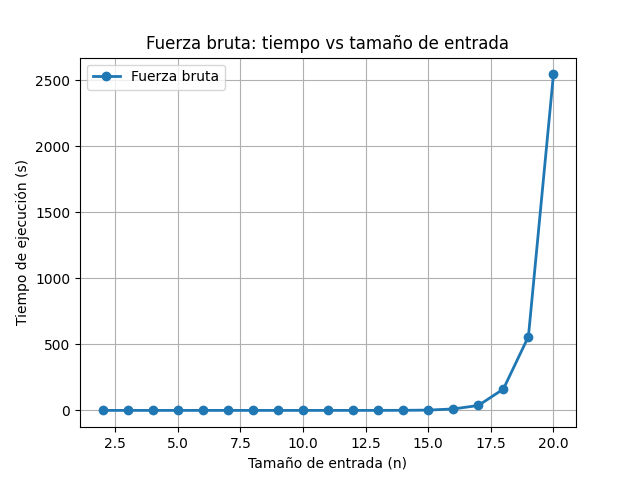
\includegraphics[width=0.8\textwidth]{code/brute_force/data/plots/brute_force_plot.png}
    \caption{Tiempos de ejecución para el algoritmo de fuerza bruta.}
    \label{fig:selectionsort}
\end{figure}

Los datos obtenidos para el algoritmo de fuerza bruta revelan con mucha claridad el carácter exponencial de su tiempo de ejecución. Si se observan los puntos correspondientes a tamaños de entrada entre $n=2$ y $n=10$, los tiempos permanecen en el orden de los microsegundos, de modo que la curva luce prácticamente plana. Una vez que uno supera el largo de $n=10$, la pendiente de la curva comienza a inclinarse. Para $n=10-15$ se empieza a percibir un incremento en tiempo de ejecución. A partir de $n=16$, el comportamiento del algoritmo y su tiempo de ejecución se multiplica exponencialmente alcanzando más de 2.500 segundos. Esta aceleración casi vertical en el gráfico refleja la complejidad teórica del algoritmo: al explorar todas las subsecuencias posibles de cada cadena, el trabajo efectivo se duplica con cada carácter adicional.

\vspace{0.5 cm}

El resultado práctico es una escalabilidad nula: el algoritmo solo resulta utilizable para entradas muy pequeñas. A partir de $n=15$ o más, se vuelve poco manejable. Esta complejidad teorica tan pobre justifica el paso a enfoques más sofisticados, como lo es la programación dinámica, que reduce el problema a complejidad cuadrática permitiendo procesar cadenas de longitudes mucho mayores.

\vspace{0.5 cm}

La tabla y el gráfico no solo corroboran la validez del algoritmo de fuerza bruta, sino que también ponen de manifiesto su inviabilidad práctica y la necesidad de técnicas de optimización para cualquier aplicación que involucre secuencias de tamaño moderado.

\vspace{0.5 cm}

\textbf{Algoritmo de programación dinámica}

Para evaluar el rendimiento del algoritmo se generaron cuatro pares de cadenas idénticas en longitud para cada tamaño, desde 2 hasta 20 caracteres. Ese mismo caso se repitió sucesivamente para los diferentes tamaños. Los resultados de dichas mediciones se presentan en la tabla que sigue.

\begin{table}[H]
  \centering
  \footnotesize
  \begin{tabular}{@{}r S[table-format=1.5e1]@{}}
    \hline
    {$n$} & {Tiempo (s)} \\
    \hline
     2  & 8.2500e-06 \\
     3  & 1.6917e-05 \\
     4  & 1.0084e-05 \\
     5  & 1.0750e-05 \\
     6  & 1.4709e-05 \\
     7  & 1.4875e-05 \\
     8  & 1.5125e-05 \\
     9  & 1.6750e-05 \\
    10  & 1.8750e-05 \\
    11  & 1.2042e-05 \\
    12  & 2.5667e-05 \\
    13  & 2.1333e-05 \\
    14  & 2.3875e-05 \\
    15  & 2.4416e-05 \\
    16  & 2.5209e-05 \\
    17  & 3.0000e-05 \\
    18  & 2.6917e-05 \\
    19  & 3.6292e-05 \\
    20  & 1.8500e-05 \\
    \hline
  \end{tabular}
  \caption{Tiempos de ejecución para programación dinámica (tamaño de entrada $n$)}
  \label{tab:tiemposDP}
\end{table}

El gráfico generado se presenta en la imagen que sigue.

\begin{figure}[H]
    \centering
    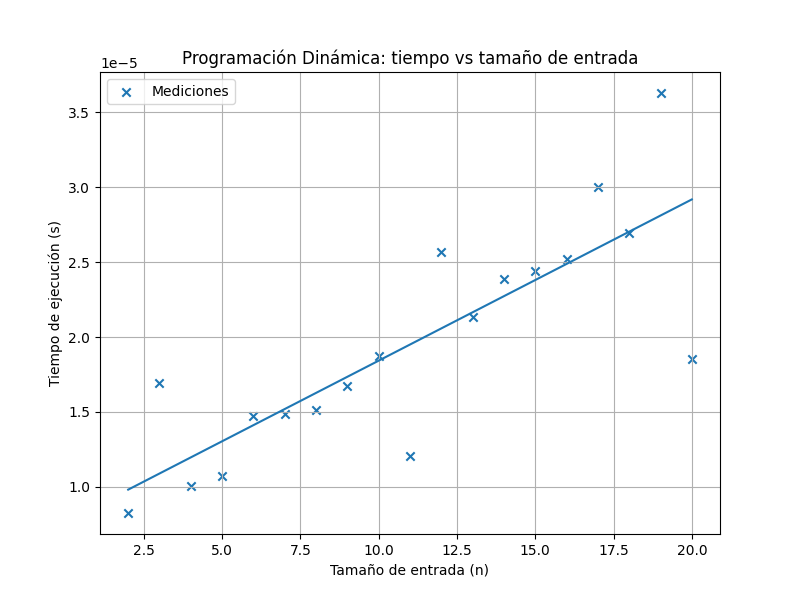
\includegraphics[width=0.8\textwidth]{code/dynamic_programming/data/plots/dynamic_programming_plot.png}
    \caption{Tiempos de ejecución para el algoritmo de programación dinámica.}
    \label{fig:selectionsort}
\end{figure}

Los datos obtenidos para el algoritmo de programación dinámica revelan con mucha claridad la eficiencia prevista para este enfoque. Todas las mediciones permanecen en el rango de los $10^{-5}$ segundos. En la práctica, el algoritmo es prácticamente instantáneo para cadenas de hasta veinte caracteres.

\vspace{0.5 cm}

El gráfico muestra que los puntos se agrupan en torno a una recta ascendente, lo que sugiere un crecimiento lineal dentro de los casos evaluados en la ejecución. Teóricamente, el algoritmo tiene complejidad cuadrática, pero con tamaños tan pequeños la parte cuadrática todavía no se vuelve dominante y la porción de la curva que alcanzamos a ver puede aproximarse razonablemente por una línea.

\vspace{0.5 cm}

Desde la perspectiva de la escalabilidad, la diferencia con la fuerza bruta es abismal. Aunque el algoritmo de programación dinámica necesita utilizar una matriz para su realización, el costo de llenarla es proporcional a $nm$ y, para los tamaños estudiados, se logran procesar en tiempos muy bajos.

\vspace{0.5 cm}

La tabla y el gráfico evidencian un algoritmo con rendimiento estable: su complejidad cuadrática no representa un obstáculo visible en este rango de entradas, y la ganancia frente a la solución de fuerza bruta justifica plenamente el uso de programación dinámica para calcular subsecuencias en aplicaciones reales.


\newpage
\section{Conclusiones}
El informe confirma la premisa planteada en la introducción: al comparar cadenas de texto, elegir bien el paradigma algorítmico marca la diferencia entre una solución altamente impractica y una herramienta realmente utilizable. Los resultados muestran que el enfoque de fuerza bruta se vuelve impracticable apenas las secuencias superan un largo de 12 carácteres, al crecer su
tiempo de ejecución de microsegundos a decenas de minutos en pocos
incrementos de tamaño. Por el contrario, la programación dinámica mantiene tiempos estables, validando en la práctica su complejidad.

\vspace{0.5 cm}

Estos hallazgos responden directamente a la premisa inicial: disponer de un método que detecte diferencias entre cadenas de forma eficiente y que escale con la longitud de entrada. Además, nos muestran la relevancia de reutilizar las subsoluciones para así lograr una mejoría ante complejidades exponenciales. En trabajos e investigaciones donde la comparación de secuencias sea una parte importante, por no decir indispensable, el paradigma
dinámico resulta completamente recomendable.

\vspace{0.5 cm}

En síntesis, el trabajo demuestra que la optimización basada en
programación dinámica logra de manera robusta los objetivos de eficiencia y escalabilidad, mientras que el paradigma de fuerza bruta es útil unicamente para instancias sumamente pequeñas. Extender este estudio a técnicas que logren reducir aún más las complejidades representa una línea natural de trabajo futuro, pero no altera la conclusión central: la selección acertada del paradigma algorítmico es el factor decisivo para abordar con éxito el problema de la comparación de secuencias.

\newpage

\section{Condiciones de entrega}
\input{condiciones}

\newpage
\appendix


\section{Apéndice 1}


\printbibliography

\end{document}


